\documentclass{article}

\usepackage{etex}               % must be include as the first package, otherwise an error will appear
\usepackage[margin=1in]{geometry}

\usepackage{float}
\restylefloat{table}

\usepackage{graphicx}
\usepackage{epstopdf}

\usepackage{url}
\usepackage{harmony}
\usepackage{musixtex}
\usepackage{subfigure}
\usepackage{caption}
\usepackage[usenames,dvipsnames,svgnames,table]{xcolor}
\usepackage{listings}
\usepackage{alltt}
\usepackage{amsmath}

\usepackage{syntax}
\renewcommand{\syntleft}{\normalfont\itshape}
\renewcommand{\syntright}{}

\usepackage{amssymb}
\usepackage{verbatimbox}

\usepackage{tikz}
\usetikzlibrary{trees}
%\usepackage{pgf}
%\usepackage{qtree}
%\usepackage{tikz-qtree}

\tikzstyle{every node}=[draw=black,thick,anchor=west]
\tikzstyle{selected}=[draw=red,fill=red!30]
\tikzstyle{optional}=[dashed,fill=gray!50]

\tikzstyle{vertex}=[draw,fill=black!15,circle,minimum size=20pt,inner sep=0pt]
\usetikzlibrary{arrows, automata, backgrounds, decorations, fit}
\usepackage[latin1]{inputenc}

\tikzset{
    fill background/.style={background rectangle/.style={fill=shadecolor},
        show background rectangle},
         data layout/.style={background rectangle/.style={fill=beige},
             show background rectangle,inner frame xsep=0pt, x=6.5pt,y=12pt},
         solidoutline/.style={very thick, draw, fill=white},
         mux2/.style={shape=trapezium, solidoutline, shape border rotate=180,
             trapezium angle=70, minimum height=8pt},
         op/.style={shape=circle, solidoutline, minimum width=12pt,
             minimum height=12pt, inner sep=0pt},
         ff/.style={shape=rectangle, fill=black, inner sep=0pt, minimum height=2pt, minimum width=8pt},
}

%\usepackage{biblatex}
%\usepackage{subcaption}

\title{\Large SMURF Programming Language Final Report} 

\author{\normalsize Richard Townsend, Lianne Lairmore, Lindsay Neubauer, Van Bui, Kuangya Zhai
	\\ \small \{rt2515, lel2143, lan2135, vb2363, kz2219\}@columbia.edu \vspace{0.6cm}}

\date{\today \vspace{2cm}}

\begin{document}

\definecolor{mygreen}{rgb}{0,0.6,0}
\definecolor{mygray}{rgb}{0.5,0.5,0.5}
\definecolor{mymauve}{rgb}{0.58,0,0.82}

\lstset{ %
	    backgroundcolor=\color{white},   % choose the background color; you must add \usepackage{color} or \usepackage{xcolor}
	    %basicstyle=\footnotesize,       % the size of the fonts that are used for the code
	    basicstyle=\scriptsize\ttfamily, 		     % the size of the fonts that are used for the code
		breakatwhitespace=false,         % sets if automatic breaks should only happen at whitespace
		breaklines=true,                 % sets automatic line breaking
		captionpos=b,                    % sets the caption-position to bottom
		commentstyle=\color{mygreen},    % comment style
		deletekeywords={...},            % if you want to delete keywords from the given language
		escapeinside={\%*}{*)},          % if you want to add LaTeX within your code
		extendedchars=true,              % lets you use non-ASCII characters; for 8-bits encodings only, does not work with UTF-8
		frame=single,                    % adds a frame around the code
		keepspaces=true,                 % keeps spaces in text, useful for keeping indentation of code (possibly needs columns=flexible)
		keywordstyle=\color{blue},       % keyword style
		language={[Objective]Caml},	     % the language of the code
		morekeywords={*,...},            % if you want to add more keywords to the set
		numbers=left,                    % where to put the line-numbers; possible values are (none, left, right)
		numbersep=5pt,                   % how far the line-numbers are from the code
		numberstyle=\tiny\color{mygray}, % the style that is used for the line-numbers
		rulecolor=\color{red},           % if not set, the frame-color may be changed on line-breaks within not-black text (e.g. comments (green here))
		showspaces=false,                % show spaces everywhere adding particular underscores; it overrides 'showstringspaces'
		showstringspaces=false,          % underline spaces within strings only
		showtabs=false,                  % show tabs within strings adding particular underscores
		stepnumber=5,                    % the step between two line-numbers. If it's 1, each line will be numbered
		stringstyle=\color{mymauve},     % string literal style
		tabsize=2,                       % sets default tabsize to 2 spaces
		title=\lstname                   % show the filename of files included with \lstinputlisting; also try caption instead of title
}

\lstdefinestyle{makefile}
{
    numberblanklines=false,
    language=make,
    tabsize=4,
    keywordstyle=\color{red},
    identifierstyle= %plain identifiers for make
}

\maketitle

\section{Introduction}

SMURF is a functional language that allows a composer to create serialist music
based on the twelve tone composition technique. In general, serialism is a musical composition
method where a set of values, chosen through some methodical progress,
generates a sequence of musical elements. SMURF is based on the
functional syntax and semantics set forth by Haskell. The backend of
SMURF generates MIDIs corresponding to the composition defined by the 
user's initial program in SMURF. 


\subsection{Background: What is Serialism?}

In general, serialism is a musical composition technique where a set of values, chosen through some 
methodical process, generates a sequence of musical elements. Its origins are often attributed to
Arnold Schoenberg's twelve-tone technique, which he began to use in the 1920s. In this system, 
each note in the chromatic scale is assigned an integer value, giving us a set of twelve
``pitch classes'' (Figure~\ref{fig:pc}~\cite{appleby2013accidentals}). A composer utilizing this 
method then takes each of these integers, and orders them into a $twelve$ $tone$ $row$, where 
each number appears exactly once. We refer to this row as the $prime$ $form$ of a piece, 
and conventionally refer to it as $P_0$. 

\begin{figure}
\begin{minipage}{0.6\textwidth}
	\centering
	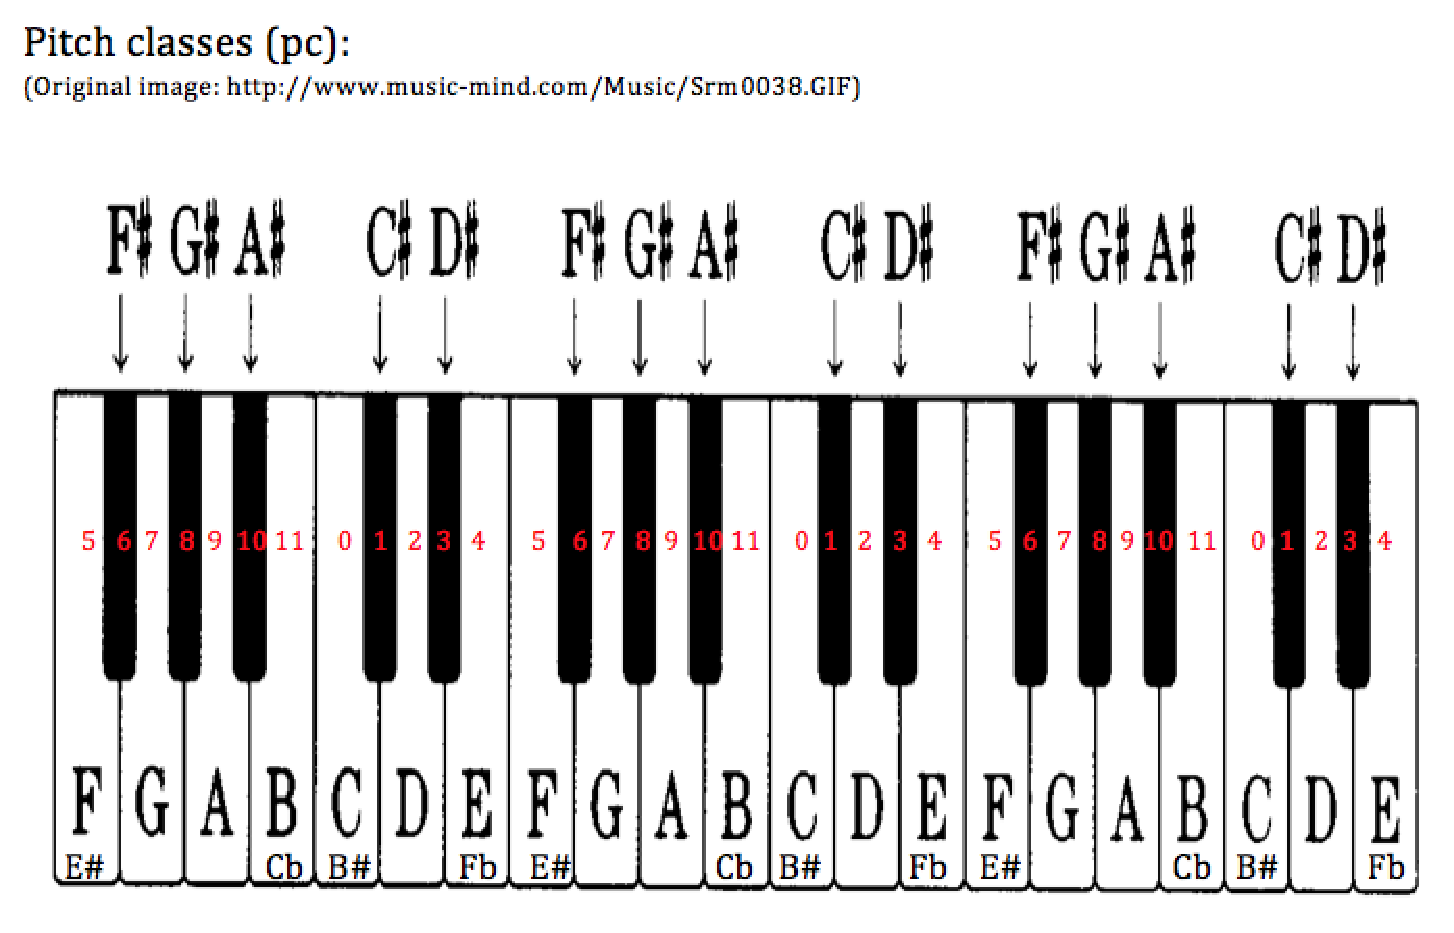
\includegraphics[width=\textwidth]{figures/serialismPianoImage}
	\caption{pitch classes}
	\label{fig:pc}
\end{minipage}\hfill
\begin{minipage}{0.4\textwidth}
	\centering
		\includegraphics[width=\textwidth]{figures/12_tone}
	\caption{twelve tone matrix}
	\label{fig:12tone}
\end{minipage}
\end{figure}


The composer can then generate other rows that are derived from $P_0$ through three types of transformations:
transposition, inversion, and retrograde. In each of these transformations, we always use mod 12 arithmetic to preserve the 
numbering system of our pitch classes. Transposing a row consists of taking each pitch class in the row and adding the same number 
to each. If we transpose $P_0$ by four semitones, we add four mod twelve to each pitch class in $P_0$ and end up with a new row 
called $P_4$. In general, $P_x$ is a transposition of $P_0$ by $x$ semitones. To invert a row, we "flip" each interval between two 
pitch classes in that row. An interval is best thought of as the smallest "distance" between two pitch classes, using the proximity
on the piano of the two pitch classes as the distance metric (refer to Figure 1 for reference). 
For example, pitch classes 0 and 11 have a distance of 1 from each other,
since you can reach pitch class 0 from 11 by adding 1 to 11 (remember the mod 12 arithmetic) or reach 11 from 0 by subtracting 1
from 0. Thus an interval of +1 exists from 11 to 0, and an interval of -1 exists from 0 to 11.
As a further example, if $P_0$ starts with pitch classes 0-11-7, then we have an interval of -1 between the first two 
pitches and -4  between the second two. Flipping an interval between two pitch classes is identical to
negating its sign.
Thus, in the inverse of $P_0$ (called $I_0$), the first interval would be +1 and the second would 
be +4, giving us 0-1-5 as our first three pitch classes.  The subscript of $I_x$  refers both to the number of transpositions required 
to arrive at $I_x$ from $I_0$, and to the prime row $P_x$ that would need to be inverted to generate $I_x$. The final row 
operation is a retrograde transformation, which merely consists of reading a row backwards. That is, $R_x$ is generated by reading 
the pitch classes of $P_x$ in their opposite order. One can also have a retrograde inversion; $RI_x$ is generated by reading the 
pitch classes of $I_x$ backwards.

Once a composer chooses a $P_0$, the three transformations outlined above can be applied to varying degrees to generate a 
$twelve$ $tone$ $matrix$, which will contain each $P$ row as a row in the matrix and each $I$ row as a column.
Furthermore, all of the $R$ and $RI$ rows are found by reading the rows in the matrix from right to left or the columns 
from bottom to top, respectively. An example of a twelve tone matrix from one of Shoenberg's pieces can be found in 
Figure~\ref{fig:12tone}~\cite{devoto2013twelve}. Finally, using the twelve tone matrix as a guide, the composer picks 
various rows and columns to serve as melodic and harmonic elements in their composition, resulting in a piece of serial music.

\subsection{Motivation}

Twelve tone serialism is a mathematically intensive method of creating music which 
involves mapping notes to numbers. It is natural to work with twelve tone rows 
using a programming language since the method treats notes like numbers that 
can be added and subtracted. SMURF makes twelve tone composition 
easier by using data types and programming paradigms that cater to the needs of a serial composer.
By simplifying the method of inverting, retrograding, and transposing rows, composers can focus 
more on how to exploit new ways to make serial music and worry less about 
creating matrices. 

We chose to implement a functional language because of the clear and 
succinct programs that functional languages produce. In addition, the well known ability
of functional languages to work on lists is advantagous for twelve tone serialism, because
most serial arithmetic operations use rows and columns from the twelve tone matrix as operands. 
As a group we were also interested on how a functional language compiler works. 

Overall we hope to use the simplicity of a functional language to help composers write 
complex, new, and interesting music based on twelve tone serialism. 

\section{Tutorial}
This tutorial covers how to install, run, and write basic SMURF programs.

\subsection{Installation} 
First, untar the SMURF tarball. To compile SMURF, simply type \texttt{make} in the top level source directory. A few sample SMURF programs are located in the \textbf{examples} directory as a reference.

\subsection{Compiling and Running a SMURF Program}
A SMURF program has the extension \textbf{.sm}. To compile and run a SMURF program, execute the \texttt{toplevel.native} file as follows:\\

\texttt{\$ toplevel.native foo.sm}\\\\
A midi file containing the composition defined in your SMURF program will generate if compilation was successful. The midi file can be played using any midi compatible software such as QuickTime. Running \texttt{toplevel.native} with the -h flag will display additional options that can be supplied to \texttt{toplevel.native} when compiling a SMURF program, such as specifying an output midi file name.

\subsection{SMURF Examples}

A basic SMURF program can generate a midi file that plays a note. The following SMURF program defines a quarter note in middle C:\\

\lstinputlisting[title=simplenote.sm]{../../Code/examples/simplenote.sm}

The identifier \texttt{main} must be set in every SMURF program. In simplenote.sm, main is set to a note.  A note in SMURF consists of a pitch class or rest, the register, and the beat. In simplenote.sm, the pitch class is set to 0, the register is 2, and the 4 indicates a single beat, which turns the note into a quarter note.

Another example TBD.

\documentclass[dvips, 12pt]{article}

% Any percent sign marks a comment to the end of the line

% Every latex document starts with a documentclass declaration like this
% The option dvips allows for graphics, 12pt is the font size, and article
%   is the style


\usepackage{etex}  % must be include as the first package, otherwise an error will appear
\usepackage[margin=1in]{geometry}

\usepackage{float}
\restylefloat{table}

\usepackage{amsmath}
\usepackage{tabularx}
\usepackage{graphicx}
\usepackage{url}
\usepackage{harmony}
\usepackage{musixtex}
\usepackage{subfigure}
\usepackage{caption}
\usepackage{listings}
\usepackage{syntax}
\usepackage{comment}
\usepackage{color}

\lstset{ %
	    basicstyle=\small\ttfamily, 
		language={Haskell},
		stepnumber=1,                    % the step between two line-numbers. If it's 1, each line will be numbered
		numbers=left,                    % where to put the line-numbers; possible values are (none, left, right)
		numberstyle=\tiny\color{black}  % the style that is used for the line-numbers
}
\renewcommand{\syntleft}{\normalfont\itshape}
\renewcommand{\syntright}{}

%\usepackage{biblatex}
%\usepackage{subcaption}

% These are additional packages for "pdflatex", graphics, and to include
% hyperlinks inside a document.


% These force using more of the margins that is the default style


% Everything after this becomes content
% Replace the text between curly brackets with your own

\title{{\Huge \bfseries SMURF Language Reference Manual} \\ \Large \it Serial MUsic Represented as Functions \vspace{0.6cm}}

\author{\normalsize Richard Townsend, Lianne Lairmore, Lindsay Neubauer, Van Bui, Kuangya Zhai
	\\ \small \{rt2515, lel2143, lan2135, vb2363, kz2219\}@columbia.edu \vspace{0.6cm}}

\date{\today \vspace{2cm}}

% You can leave out "date" and it will be added automatically for today
% You can change the "\today" date to any text you like

\begin{document}
\maketitle
\clearpage


% This command causes the title to be created in the document
\tableofcontents

\section{Introduction}
SMURF is a functional language that allows a composer to create serialist music
based on the twelve-tone composition technique. In general, serialism is a musical composition
method where a set of values, chosen through some methodical progress,
generates a sequence of musical elements. SMURF is based on the
functional syntax and semantics set forth by Haskell. The backend of
SMURF generates MIDIs corresponding to the composition defined by the 
user's initial program in SMURF. A program in SMURF, at its top-most level, 
is a series of declarations separated by newline tokens.

\section{Syntax Notation}
The syntax notation used in this manual is as follows. Syntactic 
categories are indicated by \emph{italic} type. Literal words and 
characters used in the SMURF language will be displayed in \texttt{typeset}. 
Alternatives are listed on separate lines. 

Regular expression notations are used to specify grammar patterns in this
manual.  {\it r}$*$ means the pattern {\it r} may appear zero or more times,
{\it r}$+$ means {\it r} may appear one or more times, and {\it r}$?$
means {\it r} may appear once or not at all. {\it r1}$|${\it r2} denotes an option
between two patterns, and {\it r1 r2} denotes {\it r1} followed by
{\it r2}. 


\section{Lexical Conventions}
\subsection{A High Level Description of SMURF Programs}
SMURF is a function language that allows a composer to create serialist music
based on twelve-tone composition. In general, serialism is a musical composition
technique where a set of values, chosen through some methodical progress,
          generates a sequence of musical elements. SMURF is based on the
          functional syntax and semantics set forth by Haskell. The backend of
          SMURF generates MIDIs corresponding to the uses's initial program in
          SMURF. 

\subsection{Tokens}
SMURF has 5 kinds of tokens: identifiers, keywords, constants, operators and whitespaces.

\subsubsection{Identifiers}
\label{sec:identifiers}
An identifier consists of a letter followed by other letters and
digits. The letters are the ascii characters a-z, A-Z and \_. Digits are ascii
characters 0-9. SMURF is case sensitive.
\begin{verbatim}
letter -> [`a'-`z' `A'-`Z']
digit -> [`0'-`9']
identifiers -> letter (letter | digit | `_')*
\end{verbatim}

\subsubsection{Keywords}
This is a list of reserved keywords in SMURF. The keywords are used by the
language, thus are not avaliable for re-definition or overloading.
\begin{table} [H]
	\centering
    \begin{tabularx}{0.9\textwidth}{l@{\hskip 3cm}l}
    \hline\hline
    Keywords & \\ 
    \hline\hline
      let & Specify variables and functions  \\ \hline
      in & Allow local variable binding in expression \\ \hline
      if, then, else & Specify conditional expression, else compulsory  \\ \hline
      True, False & Specify boolean logic \\ \hline
      otherwise & Specify conditional expression used with guards \\ \hline 
      %genScore & Generate musical score given list of measures as argument  \\ \hline
    \end{tabularx}
\end{table}


\subsubsection{Constants}
\label{sec:constants}
In SMURF, constants are expressions with a fixed value. Integer literials and
boolean keywords are the constants of SMURF. 

\begin{verbatim}
letter -> [`a'-`z' `A'-`Z']
digit -> [`0'-`9']
constants -> -? [`1'-`9'] digit* | True | False
\end{verbatim}


\subsubsection{Operators}
Operators in SMURF can be classied into comment operators, arithmetic operators, comparision
operators, boolean operators, list operators and function operators. 

SMURF allows nested, multiline comments in addition to single line comments.
\begin{table} [H]
\centering
\begin{tabularx}{\textwidth}{lXl}
\hline\hline
Comment Operator & Description & Example \\
\hline\hline
  /* */ & Multiline comments, nesting allowed & /* This /* is all */ commented */ \\ \hline
  // & Single-line comment & // This is a comment \\ \hline
\end{tabularx}
\end{table}

SMURF allows assignment and addition, subtraction, and modulus on expressions that evaluate to integers. These operators are all infix. The modulus operator ignores negatives e.g. 
\begin{verbatim} 13 % 12 is equal to -13 % 12 \end{verbatim}
\begin{table} [H]
\centering
\begin{tabularx}{\textwidth}{lXX}
\hline\hline
Arithmetic Operator & Description & Example \\
\hline\hline
  = & Assignment operator & a = 4 \\ \hline
  + & Integer arithmetic: plus  & a + 2 \\ \hline
  $-$ & Integer arithmetic: minus  & 5 $-$ a \\ \hline 
  \% & Integer arithmetic: modulus, ignores negatives  & 14 \% 12 \\ \hline
  $\wedge+$ & Beat add operator & 2 $\wedge+$ 2 = 1 (The add of two half notes evaluates one whole note) \\ \hline
  $\wedge-$ & Beat substract operator & 1 $\wedge-$ 2 = 2 (One whole note substracts one half note evaluates one half note) \\ \hline
\end{tabularx}
\end{table}

SMURF allows comparison operations between expressions that evaluate to integers.
\begin{table} [H]
\centering
\begin{tabular}{lll}
\hline\hline
Comparison Operator & Description & Example \\
\hline\hline
  \textless  & Less than & if a \textless\space  5 then True else False \\ \hline
  \textgreater  & Greater than & if a \textgreater\space  5 then True else False  \\ \hline
  \textless=  & Less than or equal to & if a \textless= 5 then True else False \\ \hline
  \textgreater= & Greater than or equal to & if a \textgreater= 5 then True else False \\ \hline
\end{tabular}
\end{table}


SMURF allows logical negation, conjunction, and disjunction, in addition to structural comparison and boolean notation for use with guards.
\begin{table} [H]
\centering
\begin{tabular}{lll}
\hline\hline
Boolean Operator & Description & Example \\
\hline\hline
   == & Structural comparison & if a == 5 then a = True else a = False \\ \hline
   \textcolor{red}{not} & Logical negation & if not a == 5 then True else False \\ \hline
   \&\& & Logical conjunction & if b \&\& c  then True else False \\ \hline
   \textbar\textbar & Logical disjunction & if b \textbar\textbar\space   c  then True else False \\ \hline
 \end{tabular}
\end{table}

SMURF allows concatenation and construction of lists.
\begin{table} [H]
\centering
\begin{tabular}{lll}
\hline\hline
List Operator & Description & Example \\
\hline\hline
   ++ & Concatenation: concat & [1,2,3] ++ [4,5,6] (result is [1,2,3,4,5,6]) \\ \hline
   : & Construction: cons & 1 : [2,3,4] (result is [1,2,3,4]) \\ \hline
   $[]$ & List constructor & $[]$ (result is an empty list) \\ \hline
\end{tabular}
\end{table}


SMURF allows type, argument, and function return type specificatio in addition
to concatenation and construction operations.
\begin{table} [H]
\centering
\begin{tabularx}{\textwidth}{lXl}
\hline\hline
Function Operator & Description & Example \\
\hline\hline
   :: & Type specification & returnIntFunc :: Int \\ \hline
   \textendash\textgreater & Argument and function return type specification
     & isPositiveNum :: Int \textendash\textgreater\space Bool  \\ \hline
   \textbar & Boolean operator used with guards & isSeven num :: [Int] \textendash\textgreater\space Bool\\ 
     && \textbar\space (num == 7) = True \\
     && \textbar\space otherwise = False\\ \hline
\end{tabularx}
\end{table}

SMURF allows 3 transformation operations to tone rows: inversion, retrograde and
transposition.
\begin{table} [H]
\centering
\begin{tabularx}{0.9\textwidth}{llX}
\hline\hline
Tone Row Operator & Description & Example \\
\hline\hline
   $\sim$ & Inversion & $\sim$ {\it row} (returns the inversion of {\it row})\\ \hline
   \textless\textgreater & Retrograde & \textless\textgreater~{\it row} (returns the
           retrograde of {\it row})\\ \hline
   $\wedge\wedge$ & Transposition & $\wedge\wedge$ {\it row} 3 (transposes {\it row} by 3
           semitones)\\ \hline
\end{tabularx}
\end{table}


\subsubsection{Whitespace}
Blanks, tabs and newlines are referred to as whitespaces in SMURF. SMURF treats
\texttt{newlines} as tokens and ignores others whitespaces. 


\subsection{Separators}
SMURF uses separators to seperate tokens. The separators of SMURF include:
\begin{verbatim} 
    ,   :   ;   {   }   whitespaces
\end{verbatim}


\section{Meaning of Identifiers}
In SMURF, identifiers refer to functions and variables.

\subsection{What Are They Need For}
\subsubsection{Functions}
Functions in SMURF enable us to structure our programs in a more modular way. 
A function is a group of statements that is executed when it is called from some
point of the program. 

\subsubsection{variables}
In SMURF, a variable is an abstraction of a computer memory cell or a collection
of memory cells. 
SMURF is a strongly typed programming language, which means the type of a variable can't
be changed once declared. Each variable has a static type which is automatically
deduced by the SMURF compiler. The variables in SMURF are immutable.

\subsection{Scope and Lifetime}
In SMURF, a variable is bound in its scope to a value using constructs like
\texttt{let} or list comprehensions. A variable is visible within its scope.
There is no global variables in SMURF. A variable becomes invalid after the 
ending of its scope.

\subsection{Basic Types}
There are two fundamental types in SMURF: int and bool. 
\begin{itemize}
\item Integer: \texttt{int}, used to represent integers.
\item Boolean: \texttt{bool}, used to represent boolean values.
\end{itemize}

\subsection{Structured Types}
Structured types hold groups of elements. There are three structured types in
SMURF: tuples, lists and functions.

Tuples have the format of 
\begin{verbatim}
(a, ..., n)
\end{verbatim}
where items \texttt{a - n} are elements in the tuple. Elements
of tuples can have different types.

Lists have the format of 
\begin{verbatim}
[a, ..., n]
\end{verbatim}
where items \texttt{a - n} are elements in the list. Elements
of lists must have the same type.

Functions have the format of 
\begin{verbatim}
arg1 -> arg2 -> ... -> argk -> return-value
\end{verbatim}
where \texttt{arg1 - argk} are the types of arguments of function.


\subsection{Derived Types}
SMURF has a derived type of \texttt{note}, which has the format of 
\begin{verbatim}
(pc, reg)^k[.]*
\end{verbatim}
where \texttt{pc} is an integer in the range from -1 to 11. When \texttt{pc} 
has a value of -1, the note is a rest, other it represents the pitch class of 
the note. 
\texttt{reg} is an integer in the range of 0-3, representing the register of the 
note. The register of the note is Bass 1, Bass 2, Treble 1 and Treble 2 for the
\texttt{reg} value from 0 to 3 repectively.
\texttt{k} is an integer of the power of 2, ranging from 1 to 16. 
Periods following \texttt{k} are optional. Users can add dots until the added duration
gets down to 16th note.

\begin{comment}

\subsubsection{Pitch}
pc (pitch classes) are represented by integers ranging from 0 to 11.
\begin{itemize}
  \item A Note with pc = -1 represents a rest. In this special case, the register for the Note only matters in relation
  to whether the rest lies on the treble or bass clef (i.e. whether the register is positive or negative)
\end{itemize}

\subsubsection{Beat}
A Beat represents a length of musical time. It has a Time tag and integer type. 
\begin{itemize}
  \item Must have the string ``Time" followed by an integer that is a power of 2 and \textless\space 32 in declaration
  \begin{itemize}
    \item whole note: Time 1
    \item half note: Time 2
    \item quarter note: Time 4
    \item eighth note: Time 8
    \item sixteenth note: Time 16
    \item thirty-second note: Time 32
  \end{itemize}
  \item Uses + operator to combine Time but only adds two operands that contain the same integer; recursively 
  checks for Time operands that contain the same integers until only unequal Time integers are left
  \begin{itemize}
    \item Time 4 + Time 16 + Time 16 + Time 16 + Time 16
    \item Time 4 + Time 8 + Time 16 + Time 16
    \item Time 4 + Time 8 + Time 8 
    \item Time 4 + Time 4 = Time 2 (quarter note + quarter note = half note)
  \end{itemize}
\end{itemize}

\subsubsection{Register}
Registers are represented by integers ranging from 0 to 3.
\begin{itemize}
  \item \begin{music}  \trebleclef  \end{music}  Treble Clef: notes middle C and
  higher represented by 2 and 3  
    \begin{itemize}
    \item middle C to the first B above middle C: 2 
    \item first C above middle C to next highest B: 3
    \end{itemize}
  \item \begin{music} \bassclef  \end{music}  Bass Clef: notes lower than middle
  C represented by 0 and 1 
    \begin{itemize}
    \item B directly below middle C to first C below middle C: 0
    \item next lowest B to next lowest C: 1
    \end{itemize}
\end{itemize}

\subsubsection{Note}
A Note is a tuple of three integers and is declared as 
\begin{verbatim}
(pc: int, beat: Beat, register: int)
\end{verbatim}

\subsubsection{Chord}
A Chord is a list of notes and is declared as [Note]. The compiler will check that all notes in the list have 
the same beat count.
\end{comment}

% \subsubsection{Measure} 
% Measure are abandoned in lrm



\section{Expressions}


\subsection{Curried Applications}

    \subsubsection{Function declaration}
    The syntax of a function declaration is as follows: 
    \begin{verbatim} 
    function-expression :: argument-type-list -> result-type 
    \end{verbatim} 
    where
    \begin{verbatim}
    argument-type-list:     argument-type
                            argument-type-list  argument-type
    \end{verbatim} 
A function declaration must be on its own line and must declare a type. Declaring a general type is allowed. There are no explicit return statements.
  
    \subsubsection{Function application}
    The syntax of a function application is as follows: 
    \begin{verbatim}
    function-expression  argument-expression-list \end{verbatim} 
    where
    \begin{verbatim}
    argument-expression-list:     argument-expression
                                  argument-expression-list  argument-expression
    \end{verbatim} 
A function application associates from left to right, so parentheses are optional: 
    \begin{verbatim}
    funct a b
    \end{verbatim}
    is equivalent to
    \begin{verbatim}
    ((funct a) b) 
    \end{verbatim}
    Parentheses are used to change the precedence from the default. The following evaluates funct1 with argument b then evaluates funct2 with argument a:
    \begin{verbatim}
    funct2 a (funct1 b)
    \end{verbatim}   

  \subsubsection{**PARTIAL APPLICATION**}
  

\subsection{Operator Application}
  The syntax for applying a binary operator to two expressions is infix:
    \begin{verbatim}
    expression  operator  expression \end{verbatim} 
    where
    \begin{verbatim}
    operator:     arithmetic-operator
                  comparison-operator
                  boolean-operator
                  list-operator
                  function-operator \end{verbatim} 

\subsection{Conditionals}
  The syntax for conditional expressions is as follows:
  \begin{verbatim}
  if  expression  then expression-true  else expression-false \end{verbatim} 
  When the value of expression evaluates to true, expression-true is evaluated, otherwise expression-false is evaluated. Conditional expressions do not have newline restrictions.

\subsection{Lists}
Lists are written as:
  \begin{verbatim}
  [expression-list]\end{verbatim}
  where
  \begin{verbatim}
  expression-list:     <empty>
                       expression
                       expression-list,  expression \end{verbatim}
[expression$_{1}$, ..., expression$_{k}$]  =  expression$_{1}$ : ( expression$_{2}$ : (... (expression$_{k}$ : [ ] )) \\ \\
where \textit{k} \textgreater\space 0. The expressions in a list must all be of the same type. Both the list constructor : and empty list [ ] are reserved as part of the language syntax and therefore cannot be hidden or redefined. The list constructor has right associativity.

\subsection{Tuples}
Tuples are written as:
  \begin{verbatim}
  (expression-list)\end{verbatim}
  where
  \begin{verbatim}
  expression-list:     expression, expression
                       expression-list,  expression \end{verbatim}
The expressions in a tuple may be of different types. The constructor of an n-tuple is denoted by (\textunderscore
, ..., \textunderscore) where there are \textit{n-1} commas.

\subsection{Parenthesized Expressions}
Parenthesized expressions has the form:
  \begin{verbatim}
  (expression)\end{verbatim}
  where expression is evaluated as a primary expression.

\subsection{Expression Type-Signature}
Expression type-signatures have the form:
  \begin{verbatim}
  expression :: type \end{verbatim}
  where expression is an expression and type is a type. This is used to explicitly define a type for an expression. The declared type may be more specific than the principal type but it is illegal to give a declared type that is more general than the principal type. Giving a declared type that is not comparable to the principal type will also yield an error.

\subsection{Let Expressions}
\begin{grammar}
<let-exp> $\rightarrow$ let <decls> in <expression>
\end{grammar}
Let expressions have the form \emph{let \{} $d_1;...;d_n$ \} \emph{in e}, where $d_n$ is the nth declaration and \emph{e} is an expression. Note that the scope of $d_n$ is in \emph{e}.

% are pattern bindings matched lazily?

\subsection{Pattern Matching}

Patterns can be found in function definitions, pattern bindings, and list operations. Patterns are matched with values. Matching a pattern can either be successful or it can fail. A successful match will return  a binding for the variables in the pattern. 

\subsection{Guards}
\begin{grammar}
<guard> $\rightarrow$  let <decls> | <infixexp>          
\end{grammar}

There are two kinds of guards in SMURF: local bindings and boolean guards. Local bindings have the form let $<decls>$ and introduces the declarations to the program environment. Boolean guards are expressions of type Bool. The boolean guard succeeds if the expression evaluates to True.


\section{Declarations and Bindings}

This section of the LRM describes the syntax and informal semantics of
declarations in SMURF. A program in SMURF, at its top-most level, is a
series of declarations. However, declarations may also occur inside of
\texttt{let} expressions. The scoping of such declarations is described 
in this sections. There are three types of declarations in SMURF: 
type signatures, pattern declarations, and function declarations.

\subsection{Type Signatures}

\begin{grammar}

<type-sig> $\rightarrow$ <identifier> :: <type>

<type> $\rightarrow$ Int | Bool | Note | [<type>] | 
										( <type>, $\ldots$, <type> ) | <type> -> <type> | ( <type> )
										

\end{grammar}

A type signature explicitly defines a type for a given identifier. The
\texttt{::} operator can be read as ``has type of." Only one type signature
for a given identifier can exist in a given scope. That is, two different
type signatures for a given identifier can exist, but they must be declared
in different scopes. There are three categories of types in SMURF: primitive
types,  structured types, and type synonyms. By convention, type
names are identifiers starting with an uppercase letter.

\subsubsection{Primitive Types}

The three types \texttt{Int}, \texttt{Bool}, and \texttt{Note} are
the fundamental building blocks of the type system in SMURF. 

\subsubsection{Structured Types}

SMURF has three structured types: lists, tuples, and functions. Each
type is represented by a special syntactic construct that operates on
other types to generate a concrete structured result.

The list type is written as \texttt{[t]} which specifies the type of lists
containing elements of type t.

The tuple type is written as \texttt{$(t_1, t_2, \ldots, t_n)$} where $t_i$
can be any type. THis specifies the type of tuples of size $n$ whose first
element has type $t_1$ second element has type $t_2$, and so on. A tuple
type must have at least two elements.

The function type is written as \texttt[$t_1 -> t_2$] and specifies the type
of functions that take an argument of type $t_1$ and return a value of type
$t_2$. As with tuple types, $t_1$ and $t_2$ do not have to be the same.
The function arrow is right-associative, so \texttt[Int -> Bool -> Bool] is
equivalent semantically to \texttt[Int -> (Bool -> Int)]

\subsubsection{Type Synonyms}

Type synonyms give different names to specific types, making our language
more readable and less verbose.

The \texttt[Chord] type is equivalent to the \texttt[$[$Note$]$] type.

The \texttt[System] type is equivalent to the \texttt[$[$Chord$]$] type.

\subsection{Pattern Declarations}

\begin{grammar}

<identifier> $\rightarrow$ <expr> | <guards>

<guards> $\rightarrow$ $|$ <bool-expr> $=$ <expr> $\\n$ <guards> |
											 $|$	otherwise $=$ <expr>
\end{grammar}

\subsection{Function Declarations}

\subsection{\texttt{main} Declaration}

\section{Library Functions}

Below are the library functions that can be used in the SMURF language. 
These functions are implemented in SMURF but are available to all users 
for their convenience. Each library function will include a description 
and its SMURF definition. \newline

\noindent\textbf{Head}

The function \texttt{head} takes a list and returns the first element. 
This function is commonly used when working with lists. The head function
is available for all lists through the use of polymorphic typing. 

\begin{verbatim}
head_note :: [a] -> a
head (h:tl) = h
\end{verbatim} 


\noindent\textbf{Tail}

The function \texttt{tail} takes a list and returns the end of the list.
This function is commonly used when working with lists. 

\begin{verbatim}
tail_note :: [a] -> [a]
tail (h:tl) = tl
\end{verbatim} 


\noindent\textbf{MakeNotes}

The function \texttt{makeNotes} takes in three lists and returns a list 
of notes. The first list consists of expressions of type \texttt{Int} representing 
pitches or rests. The second list consists of expressions of type \texttt{Int}
representing the register that the pitch will be played in. The third list is a list 
of expressions of type \texttt{Beat} representing a set of durations. It is common in 
12 tone serialism to use lists of notes. This function allows the user 
to easily turn their modified rows and columns into a list of notes to add 
to their system. 

\begin{verbatim}
makeNotes :: [Int] -> [Int] -> [Beat] -> [Note]
makeNotes [] = []
makeNotes (h1:tl1) (h2:tl2) (h3:tl3) = (h1,h2)$h3:(makeNotes tl1 tl2 tl3)
\end{verbatim}

\clearpage



\end{document}

\section{Project Plan}

	\subsection{Processes}
		
		\subsubsection{Planning}
		We had a 2 hour meeting every Wednesday that everyone attended. In these meetings, organized by Richard (our benevolent dictator), we discussed project milestones, delegated responsibilities to each member of the group, designed and updated our design of SMURF, and eventually coded in meetings to allow for discussion of tricky parts of our implementation. We chose milestones based on a review of previous semesters team projects that were successful. 
				
		\subsubsection{Specification}
		Both our Proposal and LRM were completely outlined in our group meetings. Lindsay took notes for the group and pushed them to GitHub so all members had access.  We divided the outlines into equal sections to divide the writing and proof-reading responsibilities: Each group member had a portion to write and a different portion to proofread. Once we started coding, any updates that needed to be made were done by the person coding that portion of the language (regardless of who originally wrote that section of the LRM). 
		
		\subsubsection{Development}
		Each member of our group was given a slice of our language to implement from start to finish. By doing this, we minimized the issues that arise from having to wait for another group member's section of the code to be implemented before being able to start your own. We each followed a similar development process, implementing in the same order the scanner (first), parser, abstract syntax tree, semantic abstract syntax tree, and code generation (last). We used GitHub to track our code but did not utilize its branching features for coding. This was a decision we made to force our code to always be in a compilable/runnable form and to avoid large merging issues at the end of development. Because we divided the language into pieces and had complete ownership of our slice, using the LRM (which we worked on together) as the ultimate reference on how to implement our section was crucial. In the few cases where the LRM specification was unable to be implemented in the way we planned, the owner of that section chose how to most appropriately implement it and then updated the LRM and the rest of the group with the changes.
		
		\subsubsection{Testing}
		At the end of each stage of development, every group member wrote unit tests to ensure their slice of the code worked as anticipated. Our integration testing took the form of several "Hello World" style programs. Any failed tests were addressed as soon as the failure was discovered.
		
	\subsection{Style Guide}
	We conformed to the following coding conventions:
		\begin{itemize}
		\item Indentation: 4 spaces, with multiple indents to differentiate between nested blocks of code 
		\item Maximum Characters per Line: 100 (including indentation)
		\end{itemize}
	
	\subsection{Project Timeline}
	Our project timeline includes \emph{class deadlines} and self imposed deadlines.
		\begin{table}[htdp]
		\begin{tabular}{|l|l|}
		\hline
		Date & Milestone \\ \hline
		09-25-13 & \emph{Proposal due} \\
		10-07-13 & Initial LRM section written \\
		10-09-13 & Initial LRM section proofread \\
		10-27-13 & Full proofread of LRM  completed \\
		10-28-13 & \emph{LRM due} \\
		10-28-13 & Scanner and Parser completed  \\
		11-06-13 & Scanner and Parser tests completed \\
		11-20-13 & Semantic Analyzer completed \\
		11-27-13 & Semantic Analyzer tests completed \\
		12-04-13 & End-to-end "Hello World" compilation succeeds \\
		12-20-13& \emph{Final report due} \\ 
		\hline
		\end{tabular}
		\end{table}
		
	\subsection{Roles and Responsibilities}
		\begin{table}[htdp]
		\begin{tabular}{|l|l|}
		\hline
		Team Member & Responsibilities \\ 
		\hline
		Van Bui & Proposal: Examples \\
					& LRM: Write Parenthetical Expressions, Let Expressions, Type Signatures, \\
					& Pattern Matching \\
					& LRM: Proofread  Description of Precedence, Syntax Notation, Library Functions, \\ 
					& Declarations and Bindings \\
					& Code: Function Application, Let Expressions, test scripts  \\
		Lianne Lairmore & Proposal: Motivation \\
									& LRM: Write Description of Precedence, Syntax Notation, Library Functions, \\
									& Declarations and Bindings \\
									& LRM: Proofread Lexical Conventions, Primary Expressions, Meaning of Identifiers \\
									& Code: Literals, Main/Print/Random, Symbol Table/Environment, Polymorphism \\
		Lindsay Neubauer & Note Taker \\
										& Proposal: Language Description\\
										& LRM: Write Curried Applications, Operator Application, Conditionals, Lists, \\
										& Tuples \\
										& LRM: Proofread Parenthetical Expressions, Let Expressions, Type Signatures, \\ 
										& Pattern Matching \\
										& Code: Non-music operators, Notes, Beats, Music operators \\
		Richard Townsend & Group Leader \\
										& Proposal: Background \\
										& LRM:  Write Declarations and Bindings \\
										& LRM: Proofread Curried Applications, Operator Application, Conditionals, Lists, \\
										& Tuples \\
										& Code: Pattern Matching, Bindings, Function Application \\
		Kuangya Zhai & GitHub and LaTeX Go-To Person \\ 
								& Proposal: Generate Latex \\
								& LRM: Write Lexical Conventions, Primary Expressions, Meaning of Identifiers \\
								& LRM:  Proofread Declarations and Bindings \\
								& Code: MIDI generation, List operators, Conditionals, Function Application \\
		\hline
		\end{tabular}
		\end{table} 
		
	\subsection{Software Development Environment}
		We used the following tools and languages:
		\begin{itemize}
		\item Compiler Implementation: OCaml, version 4.01.0
		\item Musical Interface: MIDI, java package CSV2MIDI (uses java.sound.midi.*) ~\cite{csv2midi} 
		\item Testing Environment: Shell Scripts
		\item Version Control System: GitHub
		\end{itemize}
	
	\subsection{Project Log}
		\begin{table}[htdp]
		\begin{tabular}{|l|l|}
		\hline
		Date & Milestone \\ 
		\hline
		09-18-13 & Proposal writing sections assigned \\
						& GitHub repository setup \\
		09-25-13 & LRM timeline established \\
		10-02-13 & LRM writing and proofreading sections assigned \\
		10-11-13 & Switch from OpenGL musical score to MIDI music \\
		10-16-13 & Decided on top-level description of SMURF program \\
						& Outlined all acceptable inputs and outputs to a SMURF program \\
						& Assigned vertical slices to team members \\
		10-23-13 & Divided backend into semantic analyzer and translator modules  instead of single "compiler" \\
						& module \\
		11-06-13 & Decided to add polymorphism back into language \\
	   					& Discussed structure of Semantic Analyzer modules \\
		11-08-13 & Semantic analyzer started \\
		11-13-13 & Parser completed \\ 
		11-20-13 & Interpreter Started, changed output of semantic analyzer from sast to beefed up symbol table \\
		11-27-13 & Hello World end-to-end compilation succeeds \\
		12-04-13 & Semantic Analyzer with tests completed \\
		12-20-13 & Interpreters with all tests passing completed \\
		 				& Interesting SMURF program end-to-end compilation succeeds \\
		\hline
		\end{tabular}
		\end{table}
	

\section{Architectural Design}

\subsection{Overview}
The SMURF compiler transforms a SMURF program into a playable MIDI file.
 The compiler first scans the source file, parses 
the resulting tokens, creates an abstract syntax tree, semantically 
checks the abstract syntax tree, translates the tree into 
intermediate code and finally translates this intermediate 
representation into a MIDI file which can be played in most 
media players. 


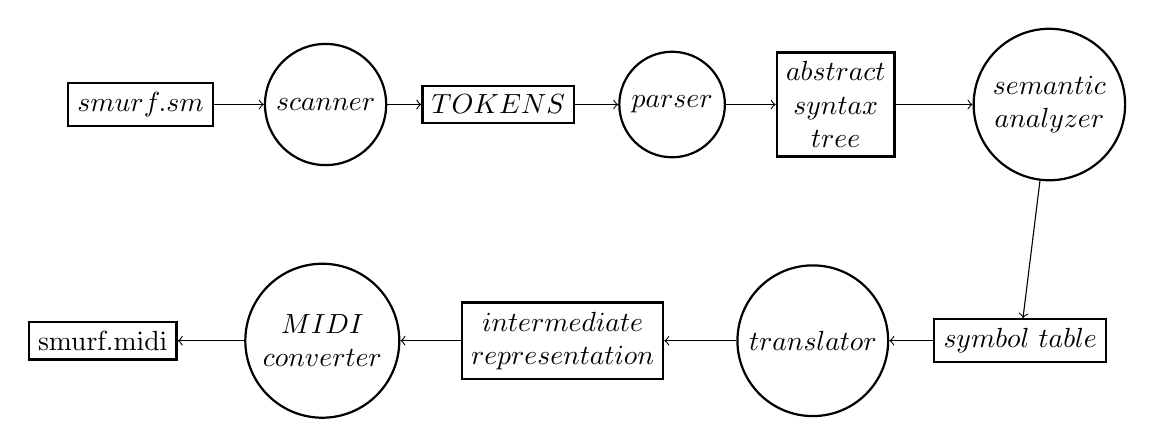
\begin{tikzpicture}[every text node part/.style={align=center}]
\node [draw,shape=rectangle] (smurf) at (0,0) {$smurf.sm$};
\node [draw,shape=circle] (scanner) at (2.5,0) {$scanner$};
\node [draw,shape=rectangle] (tokens) at (4.5,0) {$TOKENS$};
\node [draw,shape=circle] (parser) at (7,0) {$parser$};
\node [draw,shape=rectangle] (ast) at (9,0) {$abstract$ \\ $syntax$ \\ $tree$};
\node [draw,shape=circle] (semanal) at (11.5,0) {$semantic$ \\ $analyzer$};
\node [draw,shape=rectangle] (symtab) at (11,-3) {$symbol$ $table$};
\node [draw,shape=circle] (trans) at (8.5,-3) {$translator$};
\node [draw,shape=rectangle] (ir) at (5,-3) {$intermediate$ \\ $representation$};
\node [draw,shape=circle] (midic) at (2.25,-3) {$MIDI$ \\ $converter$};
\node [draw,shape=rectangle] (midi) at (-.5,-3) {smurf.midi};
\draw [->] (smurf) -- (scanner);
\draw [->] (scanner) -- (tokens);
\draw [->] (tokens) -- (parser);
\draw [->] (parser) -- (ast);
\draw [->] (ast) -- (semanal);
\draw [->] (semanal) -- (symtab);
\draw [->] (symtab) -- (trans);
\draw [->] (trans) -- (ir);
\draw [->] (ir) -- (midic);
\draw [->] (midic) -- (midi);
\end{tikzpicture}

\subsection{Scanner}
The SMURF program file is first passed to the scanner. The scanner 
matches the string of input characters to tokens and white spaces.
The tokens include keywords, constants, and operators used in a SMURF 
program. All white space characters except new lines are ignored. 
Any illegal characters are caught 
and an exception is raised. The tokens are defined with regular 
expressions and nested comments use a state machine and counter 
to be resolved. The scanner was built with the ocaml lexer. 

\subsection{Parser}
The tokens generated in the scanner are then used in the parser. 
The parser matches the string of tokens to a grammar defining the 
SMURF language. An abstract syntax tree is built as the tokens 
are matched to the grammar and stored as a program which is 
defined as a list of declarations. Syntax errors in the 
SMURF code will be identified during parsing resulting 
in an exception being raised. The parser is generated using 
the grammar and the ocaml yacc program. 

\subsection{Abstract Syntax Tree}
The abstract syntax tree is the intermediate representation 
of a SMURF program after it has been parsed but before it has 
been semantically checked. The program can easily be transversed 
by organizing the code into an abstract syntax tree because of its 
hierarchical nature. 

\subsection{Semantic Analyzer}
The semantic analyzer uses the abstract syntax tree to build a 
semantic abstract syntax tree which holds more information like 
scope and type information. Semantic errors are caught during the 
translation and transversing of the semantic abstract syntax tree. 
The semantic analyzer walked through the semantic abstract syntax tree
twice, first to create the symbol table and then to do checks using 
the filled symbol table. The second pass of the semantic abstract 
syntax tree was required because SMURF does not require variables or 
functions to be defined before they are used.  

\subsection{Translator}
The symbol table is then passed to our translator 
which evaluates all expressions and creates an intermediate 
representation that is then converted into MIDI code. 
Since symbol table contains the expression of all 
variables and functions all expressions can be evaluated 
starting from the main declaration without the semantic 
abstract symbol tree. Errors found during evaluation 
of expressions are found causing compilations errors. 
If there are no errors found then an intermediate 
representation is produced. 

\subsection{MIDI Converter}
The intermediate representation produced from the translator then 
is translated into MIDI code using the MIDI converter. The MIDI 
code can then be played. 

\section{Test Plan}

During the development process of SMURF, to let everyone envolve in the development as much as possible, we adopt the slicing model, 
i.e., in each developing stage, everyone has a slice of work to work on.
One problem with this model is that different people need to work on a same job, 
one's change to the program can easily crash other people's work. 
As a result, extensive tests to ensure the quality of the software is crucial. 


The hierachy for SMURF test cases is shown in (figure~\ref{fig:testDir}). 
In each developing stage, everyone is in charge of a directory holding test cases constructed for the functionality he/she is working on. 
Every person needs to give the expect output for his/her test cases in the {\bf exp} directory.
We have a script for testing all the test cases in the toplevel of the direcotry running all the test cases and comparing the results with the expect results given by every owner of the cases. 
The script gives the result about how many test cases passed and which test cases failed, if any. 
Before committing his/her result to the repository, everyone need to make sure the new change passed all the other people's cases. 
For the occasions that one's work need to change the output of other people's cases, 
he/she need to check the changes are as expected, 
and then generate new expected results for the cases before committing changes to repository.


\begin{figure} [H]
\centering
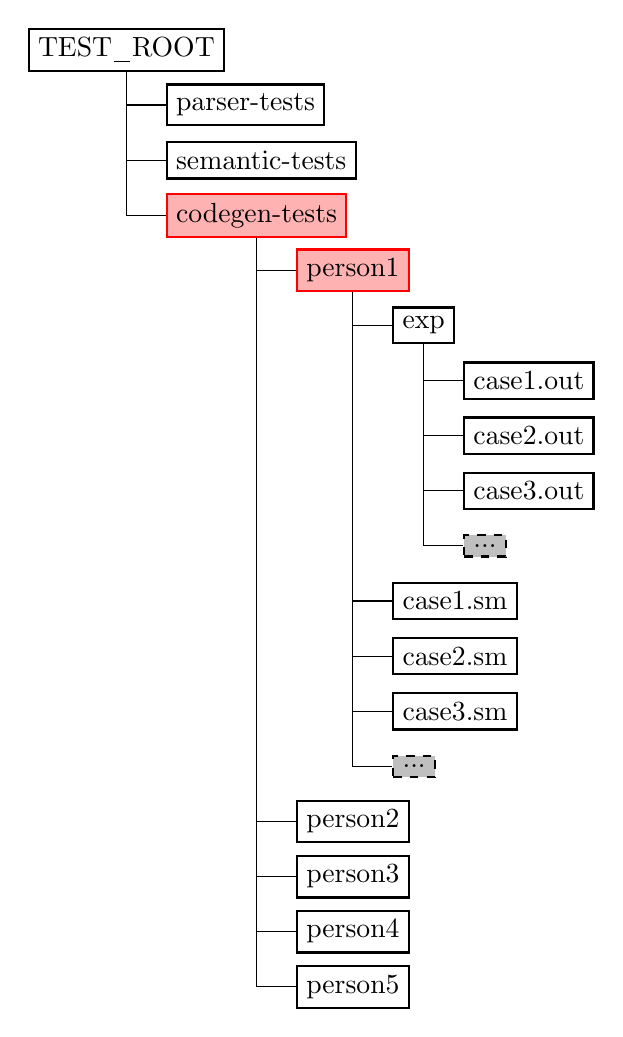
\begin{tikzpicture}[%
grow via three points={one child at (0.5,-0.7) and
    two children at (0.5,-0.7) and (0.5,-1.4)},
    edge from parent path={(\tikzparentnode.south) |- (\tikzchildnode.west)}]

    \node {TEST_ROOT}
    child { node {parser-tests}}     
    child { node {semantic-tests}}
    child { node [selected] {codegen-tests}
        child { node [selected] {person1}
            child{ node {exp}
                child{ node {case1.out} }
                child{ node {case2.out} }
                child{ node {case3.out} }
                child{ node [optional] {...} }
            }
            child [missing] {}              
            child [missing] {}              
            child [missing] {}              
            child [missing] {}              
            child{ node {case1.sm} }
            child{ node {case2.sm} }
            child{ node {case3.sm} }
            child{ node [optional] {...} }
        }
        child [missing] {}              
        child [missing] {}              
        child [missing] {}              
        child [missing] {}              
        child [missing] {}              
        child [missing] {}              
        child [missing] {}              
        child [missing] {}              
        child [missing] {}              
        child { node {person2}}
        child { node {person3}}
        child { node {person4}}
        child { node {person5}}
    };
\end{tikzpicture}
\caption{The direcotry of SMURF test cases}
\label{fig:testDir}
\end{figure}

\subsection{Testing Levels}

\subsection{Test Automation}

\subsection{Example Test Cases}
Below we give several sample test cases and their expected output for SMURF.
\subsubsection{parser-tests}
\lstset{ language=[Objective]Caml }
\lstinputlisting{../../Code/tests/parser-tests/kyzhai/test1.sm}

\subsubsection{semantic-tests}
\lstset{ language=[Objective]Caml }
\lstinputlisting{../../Code/tests/parser-tests/kyzhai/test1.sm}

\subsubsection{codegen-tests}
\lstset{ language=[Objective]Caml }
\lstinputlisting{../../Code/tests/parser-tests/kyzhai/test1.sm}

\section{Lessons Learned}

\subsection{Lindsay Neubauer}
We had a meeting at the same time every week that lasted between one and two hours that everyone attended. This time set aside to make real progress on project was crucial to our success. In the beginning of the semester we spent all the time discussing LRM-related topics and during the latter half of the semester it was split between discussion and coding. Often being in the same room, even for a short amount of time, while coding was helpful for figuring out the trickier aspects of our language. This was particularly helpful for me because OCaml was my first experience using a functional programming language and having access to others with more experience helped me pick it up quicker.
\\ \\
Another important choice we made was to designate a group leader at the beginning of this project. Our group leader was organized with tasks to discuss or complete in each meeting and helped drive the conversation in a productive way. In addition to this, we had a note taker and a person in charge of our GitHub and Latex environments. It was helpful to have �go to� people for questions and concerns that arose throughout the project.
\\ \\
After turning in our LRM we decided to divide each part of our language into slices. Each group member was in charge of a different aspect of our language and implemented that slice for each step of the compiler building process. This ownership of a part of the language was helpful and touching each step of the compiler was very helpful for learning. It also allowed each group member to work throughout the semester regardless of the progress made by others.
\\ \\
The most important learning I had from this project are understanding the functional language paradigm and knowledge on how to implement a compiler from start to finish.

\subsection{Kuangya Zhai}
First of all, the best lesson I learnt from this project is: Finish early. The importance of starting early has been told by numerous previous PLT groups while the importance of finishing early has not. By finishing early I mean you should project the finishing time of the deadline of your project a bit earlier than the actual deadline to allow any exceptions. As is always said, deadline is the first productivity. Your efficiency boosts when the deadline approaching. But there exists the possibility that something unexpected happens and you are not going to be able to finished the project in the due day if your plan is to finish everything in the last day. These situation is common when you are working on a group project. Take our group as an example, we projected everything to be finished on the exact morning of the presentation while it turned out that not everything goes well as expected, so we had to presented an incomplete version which was kind of embarrassing. And the problems was solved on the exact afternoon of the presentation but we had no chance the present it again. Had we project our own deadline one day earlier, I believe the result will be much better. 

The second thing, enjoy OCaml. Few people has functional programming background before the PLT class. So it's likely that you will have a steeper learning curve when comparing with learning other programming languages. However, when you got used to the functional style, you will find it's at least as expressive and productive as imperative languages you have got used to. The thing I love the most about functional programming is its type checking system. So you will spend tons of time to get your program to compile. But once after that, your program will likely to give the correct result since most of the bugs have been captured at the compiling stage. Also, the side effect free property of functional program guarantees the robustness of your program, which is especially important when you are working on a teaming working project. OCaml is not purely functional. It also keeps several imperative features which might also be helpful and make your life much easier when comparing with Haskell, the pure functional programming language. 

\section{Appendix}


\lstset{ language=[Objective]Caml }

\lstinputlisting{../../Code/scanner.mll}

\lstinputlisting{../../Code/parser.mly}


% commented to save compiling time
\begin{comment}
\end{comment}

\lstinputlisting{../../Code/ast.ml}
\lstinputlisting{../../Code/interpreter.ml}
\lstinputlisting{../../Code/output.ml}
\lstinputlisting{\detokenize{../../Code/parser_test.ml}}
\lstinputlisting{../../Code/sast.ml}
\lstinputlisting{../../Code/semanalyze.ml}
\lstinputlisting{\detokenize{../../Code/semantic_test.ml}}
\lstinputlisting{../../Code/toplevel.ml}
\lstinputlisting{../../Code/util.ml}
\lstinputlisting{../../Code/values.ml}

\lstinputlisting{../../Code/makefile}
\lstinputlisting{../../Code/build.mk}



\clearpage

\bibliographystyle{ieeetr}
\bibliography{ref/refs}


\end{document}
